\documentclass[a4paper,french]{paper}
\usepackage{../../_latex_assets/villemejane_iogs_ceti}

%Informations about this document 
%------------------------------------------
\def\module{Ingénierie Electronique pour le Traitement de l'Information}
\def\moduleAbrege{6N-047-SCI / IéTI}
\def\annee{}

\def\titre{TD 5 / Corriger un "vrai" système}
\author{Julien VILLEMEJANE}

\subtitle{TD 5}
\institution{LEnsE / Institut d'Optique Graduate School}

\title{\titre}
\begin{document} 
%Beginning First Page. 
%------------------------------------------
\enteteThematiqueObligatoire{}

%Beginning Content. 
%------------------------------------------
\vspace{-1cm}
%%%%%%%%%%%%%%%%%%%


\subsection*{Système d'asservissement de position d'un faisceau LASER}

Dans ce TD, on se propose d'étudier un \textbf{système réel}, son \textbf{modèle} et son \textbf{asservissement corrigé}.

\begin{center}
	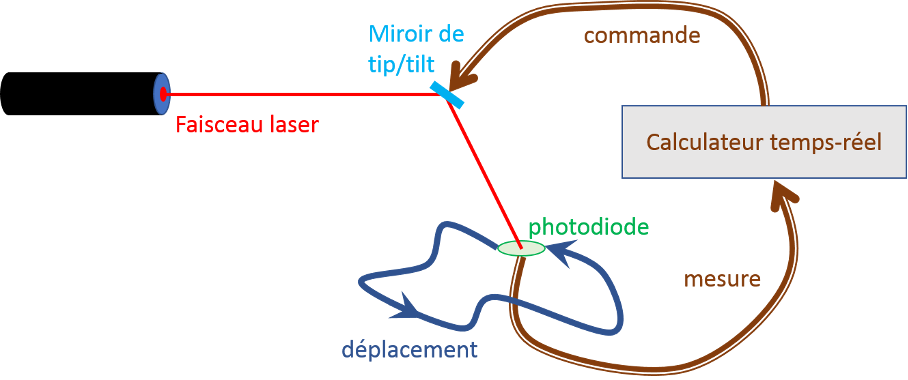
\includegraphics[width=10cm]{images/TD/systBoucle.png}
\end{center}


Le système à étudier permet de positionner un \textbf{pointeur LASER} à l'aide de deux moteurs galvanométriques selon deux directions (X et Y). L'information est récupérée par une photodiode 4 quadrants.

\begin{center}
	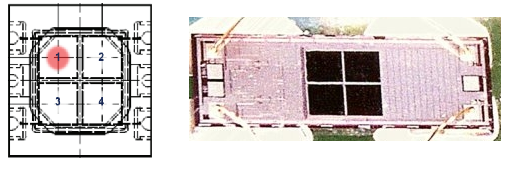
\includegraphics[width=8cm]{images/TD/4q_photodiode.png}
\end{center}

Seule la voie X sera étudiée ici, les deux directions étant équivalentes.

Les moteurs galvanométriques sont pilotés à l'aide d'une tension et asservis en angle. Pour une tension donnée le "servomoteur" se positionnera à un angle particulier.

Le capteur de position (la photodiode 4 quadrants) renvoie une tension en lien avec la position du faisceau LASER.

\subsection*{Application à l'optique adaptative}

Dans de nombreuses applications, on utilise des lasers dont le faisceau doit être pointé sur une cible avec une grande précision. Par exemple lorsque l'on crée des étoiles artificielles pour l'observation astronomique par optique adaptative, les étoiles artificielles doivent être créées à une certaine position angulaire et à une certaine altitude. La présence de l'atmosphère fait dévier le faisceau, et ces déviations peuvent être compensées par des petits miroirs plans dits de basculement (ou de tip/tilt) grâce à un asservissement utilisant la mesure des écarts à la position voulue.

\subsection*{Modèle du système}

Il a été montré expérimentalement que le système complet (servomoteur) pouvait être modélisé par la relation suivante (dans sa zone de fonctionnement linéaire) :

$$T(p) = \frac{G_0}{1 + \frac{2 \cdot m \cdot p}{w_c} + \frac{p^2}{w_c^2}}$$

Le capteur peut être modélisé par un simple gain qu'on notera $K_{capt} = 10$.

\newpage
%%%%%%%%%%%%%%%%%%%
\encadreTDExo{1 - Modèle du système}{


\begin{enumerate}
	\item Tracez le schéma bloc du système.
	\item De quel type est ce système ? Quelles sont les grandeurs d'entrée et de sortie des différents blocs ?
	
	\medskip
	
	On donne le relevé expérimental de la réponse à un échelon de ce système :
	
\begin{center}
	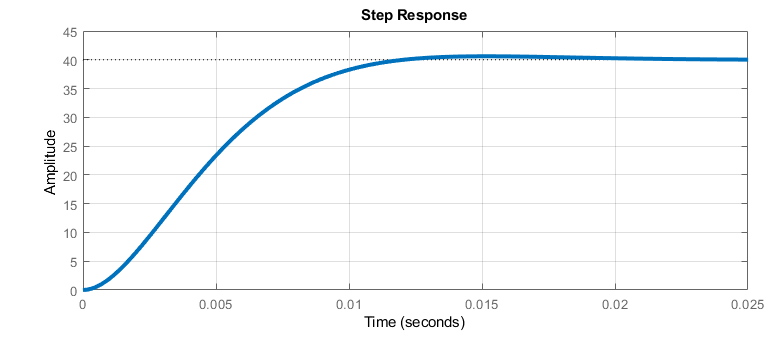
\includegraphics[width=12cm]{images/TD/step_BO.png}
\end{center}
	
	\item Identifiez le paramètre $G_0$.
	\item On obtient une valeur de $m = 0.8$ et de fréquence caractéristique $f_c = 55\operatorname{Hz}$. Est-ce cohérent avec la réponse obtenue ?
	\item Tracez le diagramme de Bode de ce système.
\end{enumerate}
}


%%%%%%%%%%%%%%%%%%%%%%%%%%%%%%%%%%%%%%%%%%%%%%%%%%%%%%%%%%%%%%%%%%
\encadreTDExo{2 - Système asservi non corrigé}{

On souhaite maintenant étudié le système asservi, sans correcteur pour l'instant ($C(p) = 1$).

\begin{enumerate}
	\item Quelle est la fonction de transfert en boucle fermée du système ?	
	\item Que valent les nouvelles caractéristiques de ce système (ordre, pulsation propre, amortissement...) ?
	\item Tracez son diagramme de Bode.
	\item La réponse à un échelon suivante est-elle celle de ce système ?
		\begin{center}
			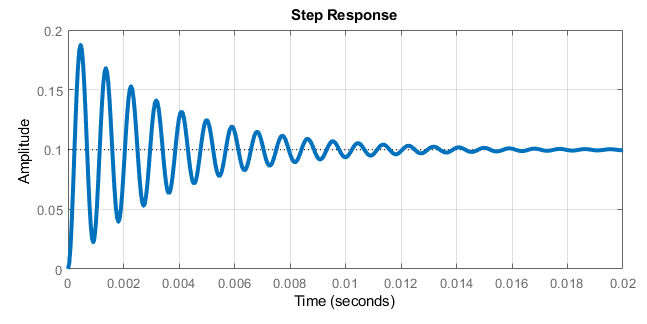
\includegraphics[width=14cm]{images/TD/step_BF.png}
		\end{center}	
\end{enumerate}
}

%%%%%%%%%%%%%%%%%%%%%%%%%%%%%%%%%%%%%%%%%%%%%%%%%%%%%%%%%%%%%%%%%%
\encadreTDExo{3 - Correcteur PID}{

On souhaite corriger ce système avec un correcteur de type Proportionnel Intégral Dérivé (PID). Une forme, dite idéale, de ce correcteur est donné par la relation suivante :

$$C(p) = K \cdot (1 + \frac{1}{K_i \cdot p} + K_d \cdot p)$$

On ne s'intéressera pas ici au réglage de ce correcteur. Il existe pour cela différentes approches, dont celle de Ziegler-Nichols. Nous allons voir quel est l'intérêt des composantes proportionnelle et intégrale d'un correcteur.

\begin{enumerate}
	\item Mettez ce système sous forme d'un schéma bloc.
	\item Donnez la forme canonique de l'expression de $C(p)$.
	\item Quelles sont les unités des coefficients $K$, $K_i$ et $K_d$ ?

	\medskip
	
	On commence par ajouter une composante $K$, les composantes intégrales et dérivées sont déconnectées.
	
	\item Que devient la fonction de transfert en boucle fermée du système asservi et corrigé ? Que deviennent les grandeurs caractéristiques de ce système ?
	\item Que valent ces valeurs pour $K = 10$ ? Pour $K = 0.1$ ?
	\item Tracez les diagrammes de Bode de ces deux systèmes sur le même diagramme que précédemment.
	
	\medskip
	
	On ajoute la composante intégrale au correcteur.
	
	\item Que devient la fonction de transfert en boucle fermée du système asservi et corrigé ? 
	
\end{enumerate}
}

\newpage

\subsection*{Correction PI}
	
	Selon le choix des coefficients $K$ et $K_i$, le système peut être corrigé, mais peut également devenir instable...
	
	\begin{center}
		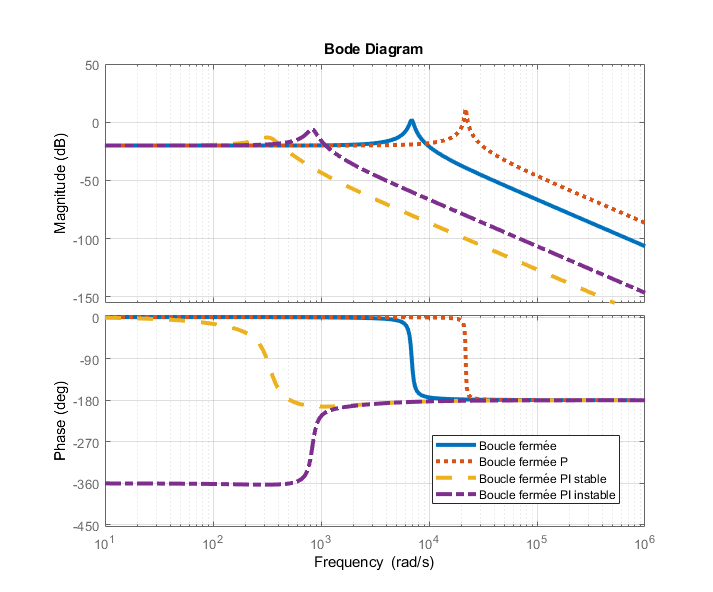
\includegraphics[width=14cm]{images/TD/bode_PI_corr.png}
	\end{center}	
	
	\begin{center}
		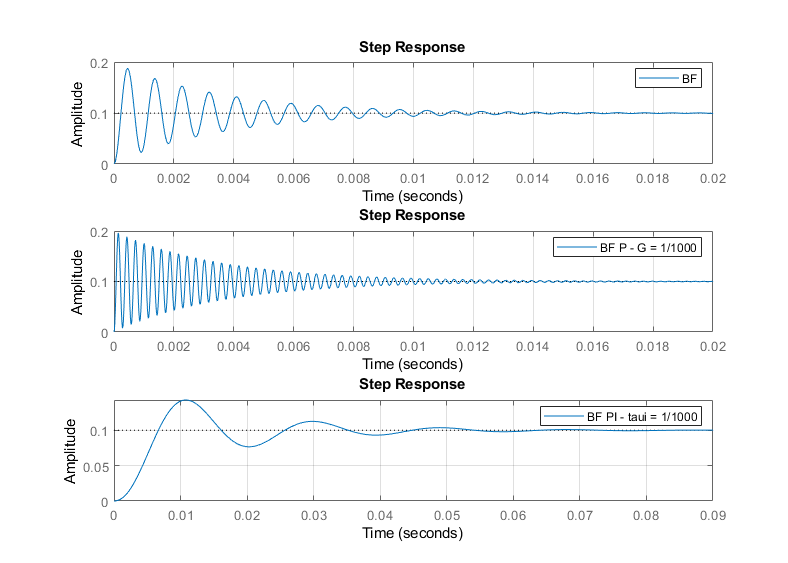
\includegraphics[width=14cm]{images/TD/step_PI_corr.png}
	\end{center}

\end {document}